\usetikzlibrary{arrows.meta,decorations.pathmorphing,matrix}

\begin{frame}<1>[fragile,label=pthreadCreateOver]{pthread\_create}
\vspace{-.25cm}
\begin{lstlisting}[
    style=smaller,
    language=C++,
    moredelim={**[is][\btHL<2|handout:2>]{@2}{2@}},
    moredelim={**[is][\btHL<3|handout:3>]{@3}{3@}},
    moredelim={**[is][\btHL<4|handout:4>]{@4}{4@}},
    moredelim={**[is][\btHL<5|handout:5>]{@5}{5@}},
]
void *ComputePi(void *argument) { ...  }
void *PrintClassList(void *argument) { ...  }
int main() {
    pthread_t pi_thread, list_thread;
    pthread_create(&@2pi_thread2@, @4NULL4@, @3ComputePi3@, @4NULL4@);
    pthread_create(&@2list_thread2@, @4NULL4@, @3PrintClassList3@, @4NULL4@);
    ... /* more code */
}
\end{lstlisting}
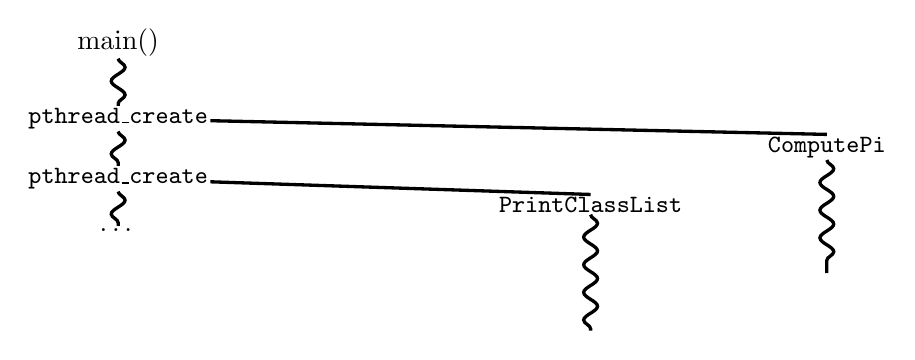
\begin{tikzpicture}
    \tikzset{
        thread/.style={very thick,draw,decorate,decoration=snake},
        split/.style={very thick,draw},
        marker/.style={thin,draw},
        y=0.8cm,
        every node/.style={inner sep=0.1mm}
    }
    \draw[thread] (0, 0) node[above] {main()}-- ++(0, -.75) node[below,font=\tt\small] (create pi) {pthread\_create};
    \draw[thread] (create pi) -- ++(0, -.75) node[below,font=\tt\small] (create list) {pthread\_create};
    \draw[split] (create pi) -- ++(9, -.25) node[below,font=\tt\small] (computepi){ComputePi};
    \draw[thread] (computepi) -- ++(0, -2);
    \draw[thread] (create list) -- ++(0, -.75) node[below] {\ldots};
    \draw[split] (create list) -- ++(6, -.25) node[below,font=\tt\small] (classlist){PrintClassList};
    \draw[thread] (classlist) -- ++(0, -2);
\end{tikzpicture}
\end{frame}

\begin{frame}[fragile,label=pthreadCreateIntro]{pthread\_create}
\begin{lstlisting}[
    style=small,
    language=C++,
    moredelim={**[is][\btHL<2|handout:2>]{@2}{2@}},
    moredelim={**[is][\btHL<3|handout:3>]{@3}{3@}},
    moredelim={**[is][\btHL<4|handout:4>]{@4}{4@}},
    moredelim={**[is][\btHL<5|handout:5>]{@5}{5@}},
]
void *ComputePi(void *argument) { ...  }
void *PrintClassList(void *argument) { ...  }
int main() {
    pthread_t pi_thread, list_thread;
    pthread_create(&@2pi_thread2@, @4NULL4@, @3ComputePi3@, @4NULL4@);
    pthread_create(&@2list_thread2@, @4NULL4@, @3PrintClassList3@, @4NULL4@);
    ... /* more code */
}
\end{lstlisting}
    \begin{itemize}
    \item pthread\_create arguments:
    \item \myemph<2>{thread identifier}
    \item \myemph<3>{function to run}
        {\fontsize{12}{13}\selectfont thread starts here, terminates if this function returns}
    \item \myemph<4>{thread attributes (extra settings) and function argument}
    \end{itemize}
\end{frame}


